\documentclass{beamer}
\usepackage[utf8]{inputenc}

\usepackage{semantic}
\usepackage{graphicx}
\usepackage{booktabs}
\usepackage{todonotes}
\presetkeys{todonotes}{inline}{}

\usepackage[absolute,overlay]{textpos}
% This is to get textpos to play well,
% A stackoverflow user mentioned that this could
% cause problems in some Acrobat Reader versions
% I'll take the chance
\usebackgroundtemplate{}


\mode<presentation> {
\usetheme{boxes} % When headline is wanted use Dresden theme instead
\usecolortheme{seagull}
\setbeamertemplate{footline}[page number]
\setbeamertemplate{navigation symbols}{}
}


%----------------------------------------------------------------------------------------
%	TITLE PAGE
%----------------------------------------------------------------------------------------

\title[APL \& TAIL] % bottom of every slide
  {Teaching kids programming, IT-creativity and modern tech} % title page

\author{\footnotesize{Martin Dybdal} \\ \footnotesize{\texttt{dybber@dybber.dk}}}

\institute {
DIKU \\
University of Copenhagen
}

\date{\footnotesize{29 April 2016}}

\begin{document}

{
\setbeamertemplate{headline}{}
\begin{frame}
  \begin{center}
    
\includegraphics[width=0.7\textwidth]{imagery/codingpirates.png}
  \end{center}
\vspace{-1cm}
\titlepage
\end{frame}
}

%----------------------------------------------------------------------------------------
%	TABLE OF CONTENTS
%----------------------------------------------------------------------------------------

\begin{frame}
\frametitle{Overview}
\tableofcontents
\end{frame}

%----------------------------------------------------------------------------------------
%	CONTENT
%----------------------------------------------------------------------------------------

\section{What is Coding Pirates?}
\begin{frame}
\frametitle{What is Coding Pirates?}
\begin{textblock}{20}(5,5)
 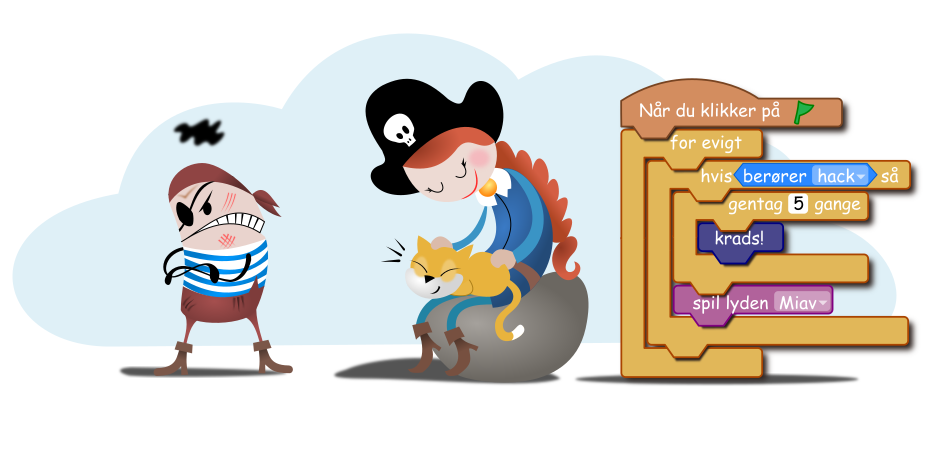
\includegraphics[width=\textwidth]{imagery/cpthack-and-miss1337-transp.png}
\end{textblock}

\begin{itemize}
\item Activity for kids aged 7-17 years
\item A creative playground - not just two more hours of school
\item Volunteer-driven organisation
\end{itemize}
\vspace{4cm}
\end{frame}

\subsection{Who are Coding Pirates?}
\begin{frame}
\frametitle{Who are Coding Pirates?}
\begin{itemize}
\item Non-profit organisation
\item +300 volunteers
  \begin{itemize}
  \item Teachers, IT professionals, researchers, librarians, IT students
  \end{itemize}
\item 1000+ kids on waiting list
\item 600+ paying members in Denmark
\item 35+ hubs in Denmark
\end{itemize}

\centerline{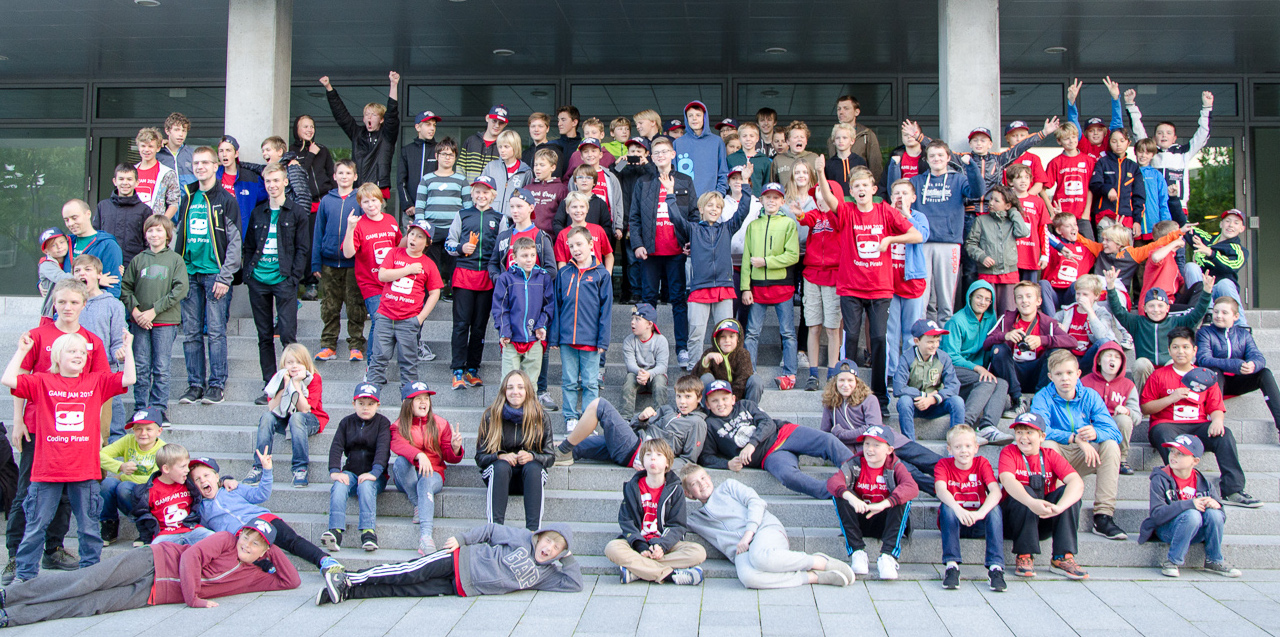
\includegraphics[width=0.9\textwidth]{imagery/gamejam}}
\end{frame}

\subsection{Motivation}

\begin{frame}
\frametitle{Motivation}

\begin{itemize}
\item Digital revolution, Information Age.
\item Democracy: New tech requires new policies. The public
  should be able to make informed decisions
\item Automatisation
\item Computational thinking is useful everywhere!
\end{itemize}
\end{frame}

\subsection{The Coding Pirates philosophy}
\begin{frame}
\frametitle{The Coding Pirates philosophy}

\begin{itemize}
\item Inspiration from Maker-movement. 
\item Curiosity, exploration
\item Accomplishment. Fight imposter syndrome
\item Computational thinking
\end{itemize}

Manifesto: \url{http://codingpirates.dk/manifesto/}

% %\vspace{5mm}
% \begin{quotation}
%   "The problems now faced by mankind are largely due to man's own
%   creativeness. Creativeness will need to account for much more if
%   present problems are to be transcended with solutions".

%   - Preface of "Explorations in Creativity", Editors: Ross L. Mooney,
%   Taher A. Razik
% \end{quotation}
\end{frame}


\section{Coding Pirates in practice}
\begin{frame}
\frametitle{In practice}

\begin{textblock}{20}(8,0.5)
 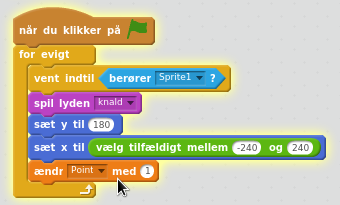
\includegraphics[width=0.3\textwidth]{imagery/scratch}
\end{textblock}

\begin{textblock}{20}(6,9)
  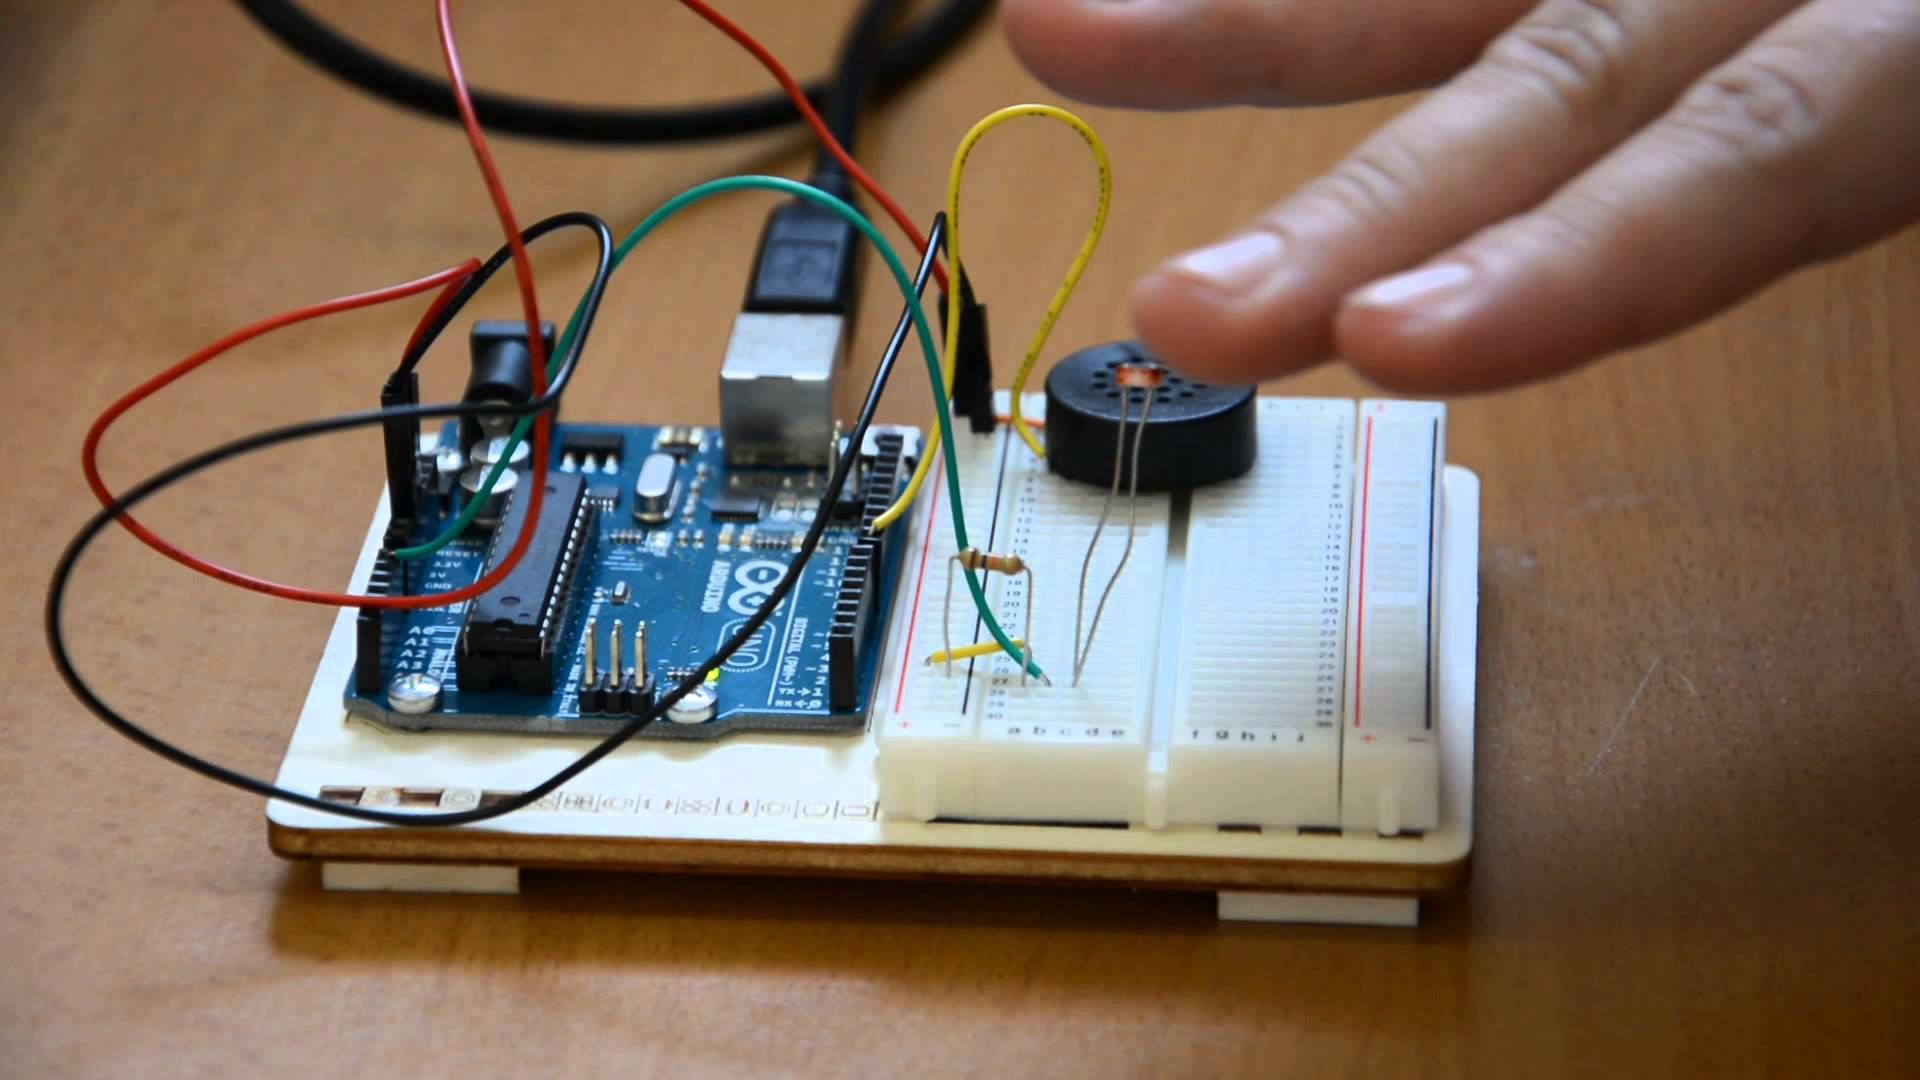
\includegraphics[width=0.4\textwidth]{imagery/arduino-theremin}
\end{textblock}

\begin{itemize}
\item $\sim$25-30 kids
\item $\sim$7-10 volunteers
\item 2 hours a week, usually 17:00-19:00
\item 15 minutes break with snacks, cool aid, fruit etc.
\item Bring your own device (BYOD)
\end{itemize}
\vspace{2cm}

\end{frame}

\begin{frame}
\frametitle{Workshops}

\begin{itemize}
\item 4-6 week workshops
  \begin{itemize}
  \item Scratch
  \item LEGO Mindstorms
  \item 3D-printing (TinkerCAD)
  \item 3D modelling in Blender
  \item Processing(.js)
  \item Arduino (Scratch or C)
  \item Unity (C\#)
  \item Python
  \item HTML/CSS
  \item ...
  \end{itemize}
\item Kids can not switch between workshops during these 4-6 weeks
\item Presentations at the end of a 4-6 week period
\end{itemize}


\end{frame}

\subsection{Showcase of projects}

\begin{frame}
  \frametitle{Example project: Horror teddy bear}
  by Penelope, 12 years
  \vspace{7mm}

  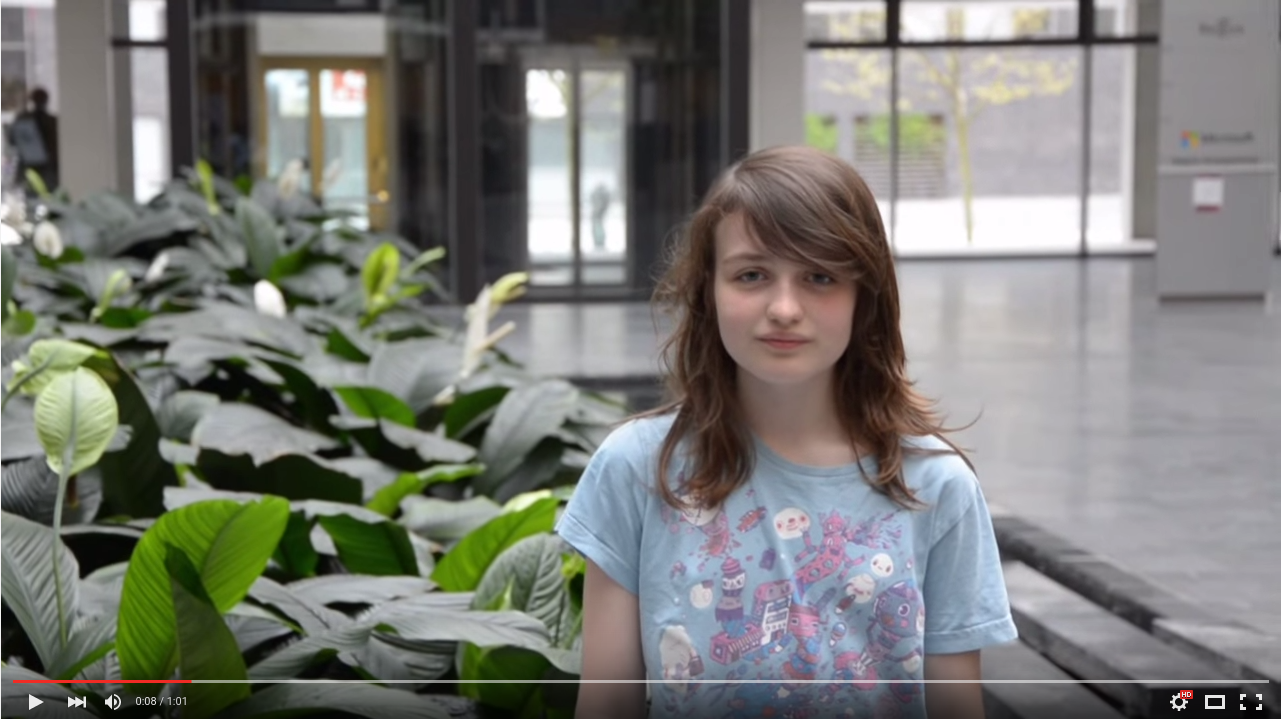
\includegraphics[width=\textwidth]{imagery/penelope-raedselsbamse}

  \url{https://www.youtube.com/watch?v=Mc21BbiUGxU}
\end{frame}



\begin{frame}
  \frametitle{Stickman dungeon}
  by Alexander and Oscar, 11 years

  \centerline{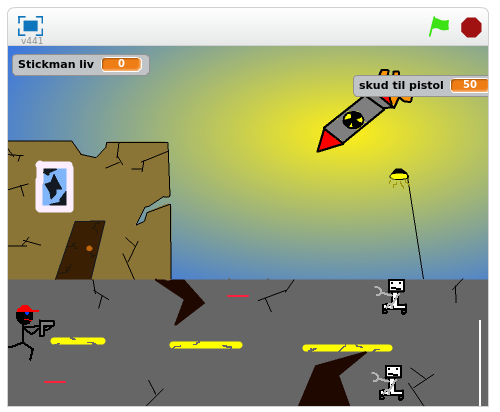
\includegraphics[width=0.8\textwidth]{imagery/stickman-dungeon}}

  \url{https://scratch.mit.edu/projects/57201286/}
\end{frame}



% \begin{frame}
%  \vspace{5mm}
%  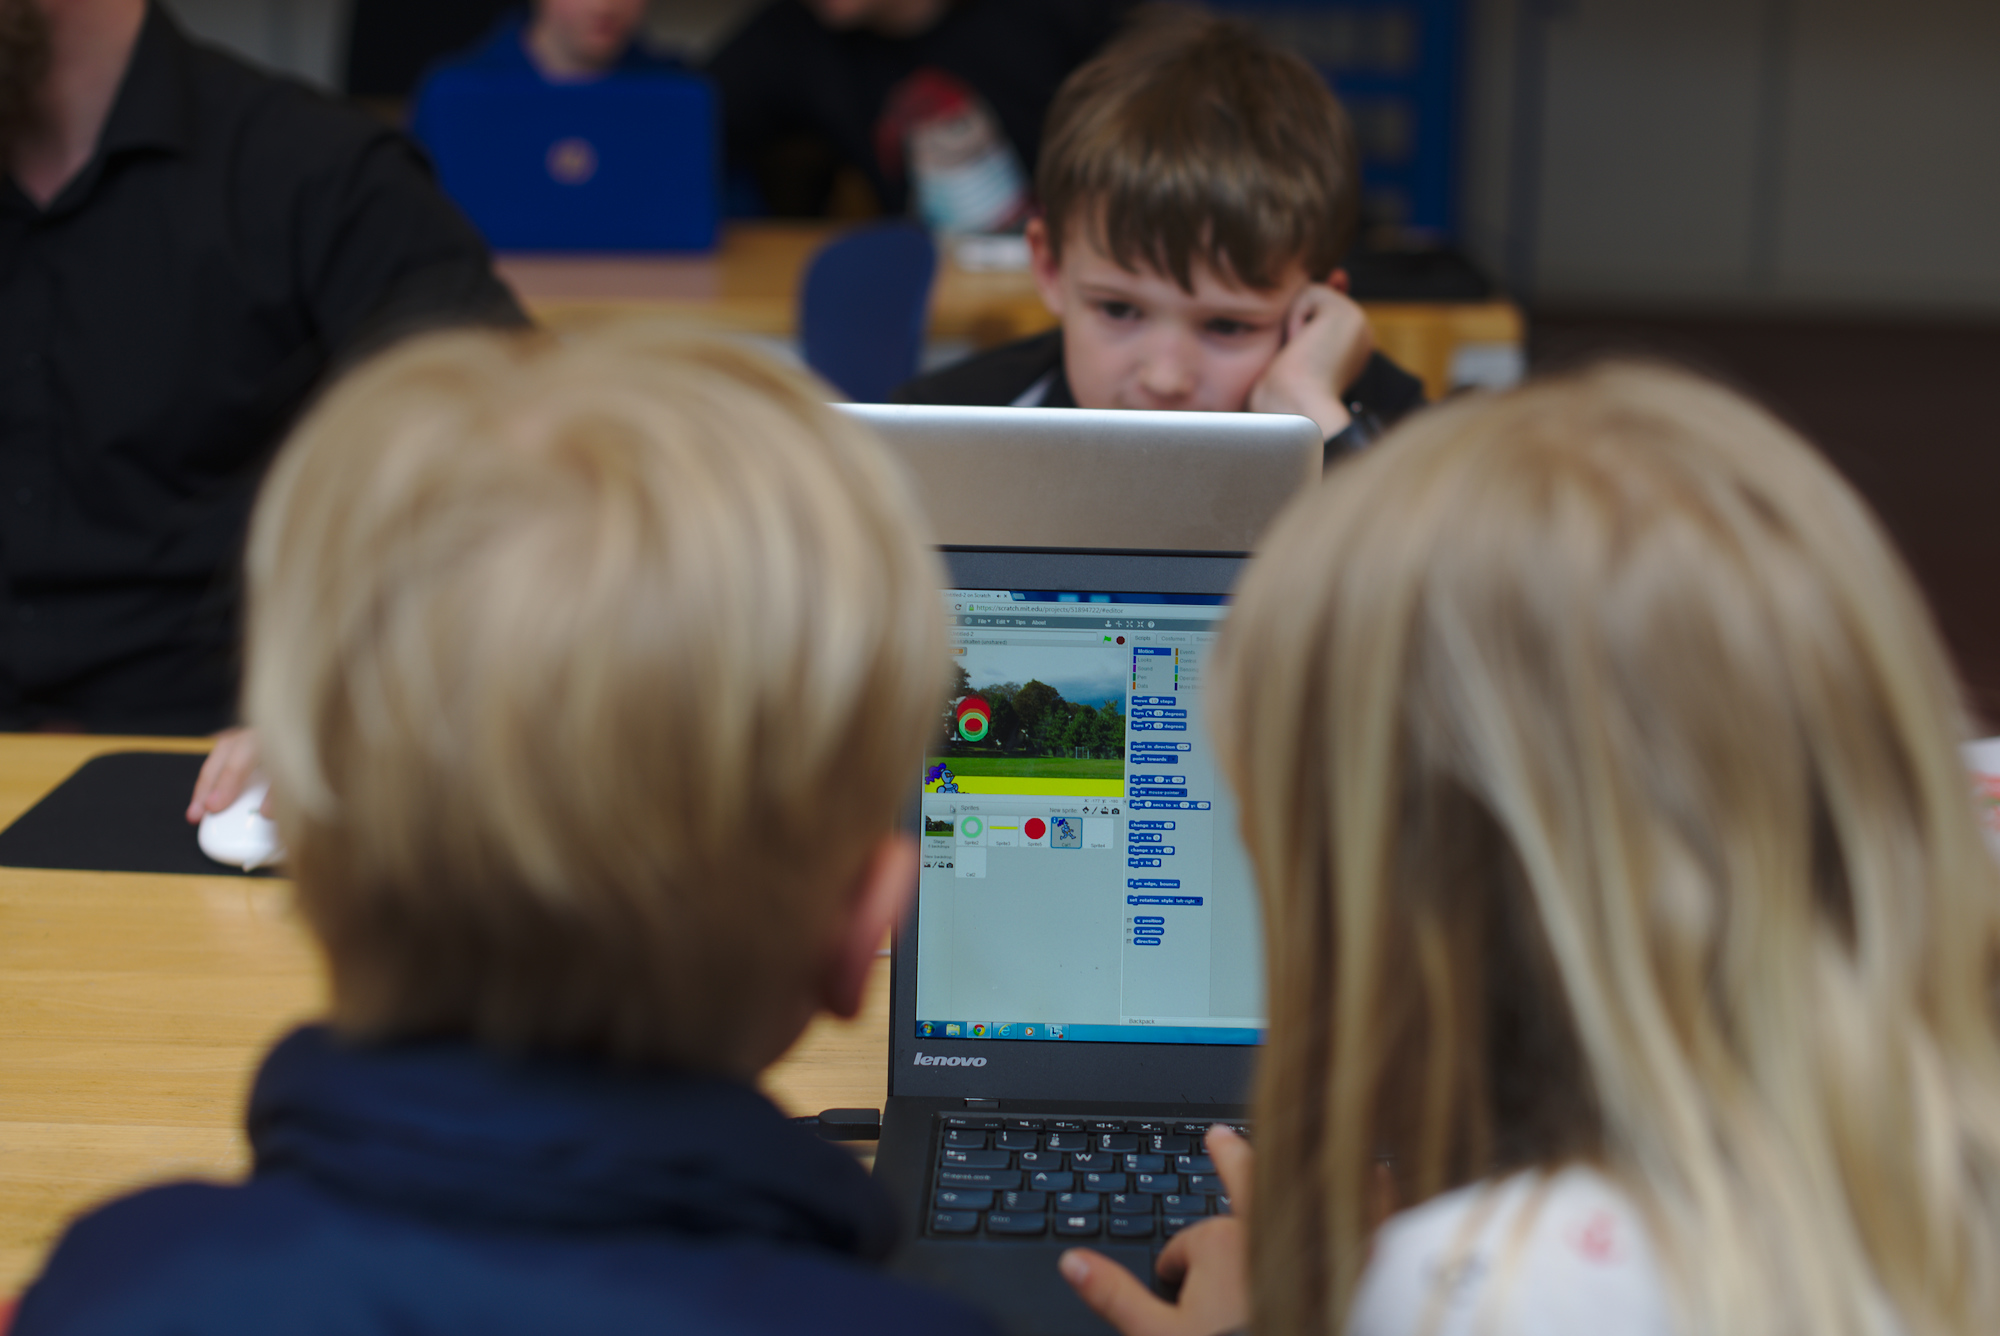
\includegraphics[width=\textwidth]{imagery/william-sofie}
% \end{frame}

\begin{frame}
 \vspace{5mm}
 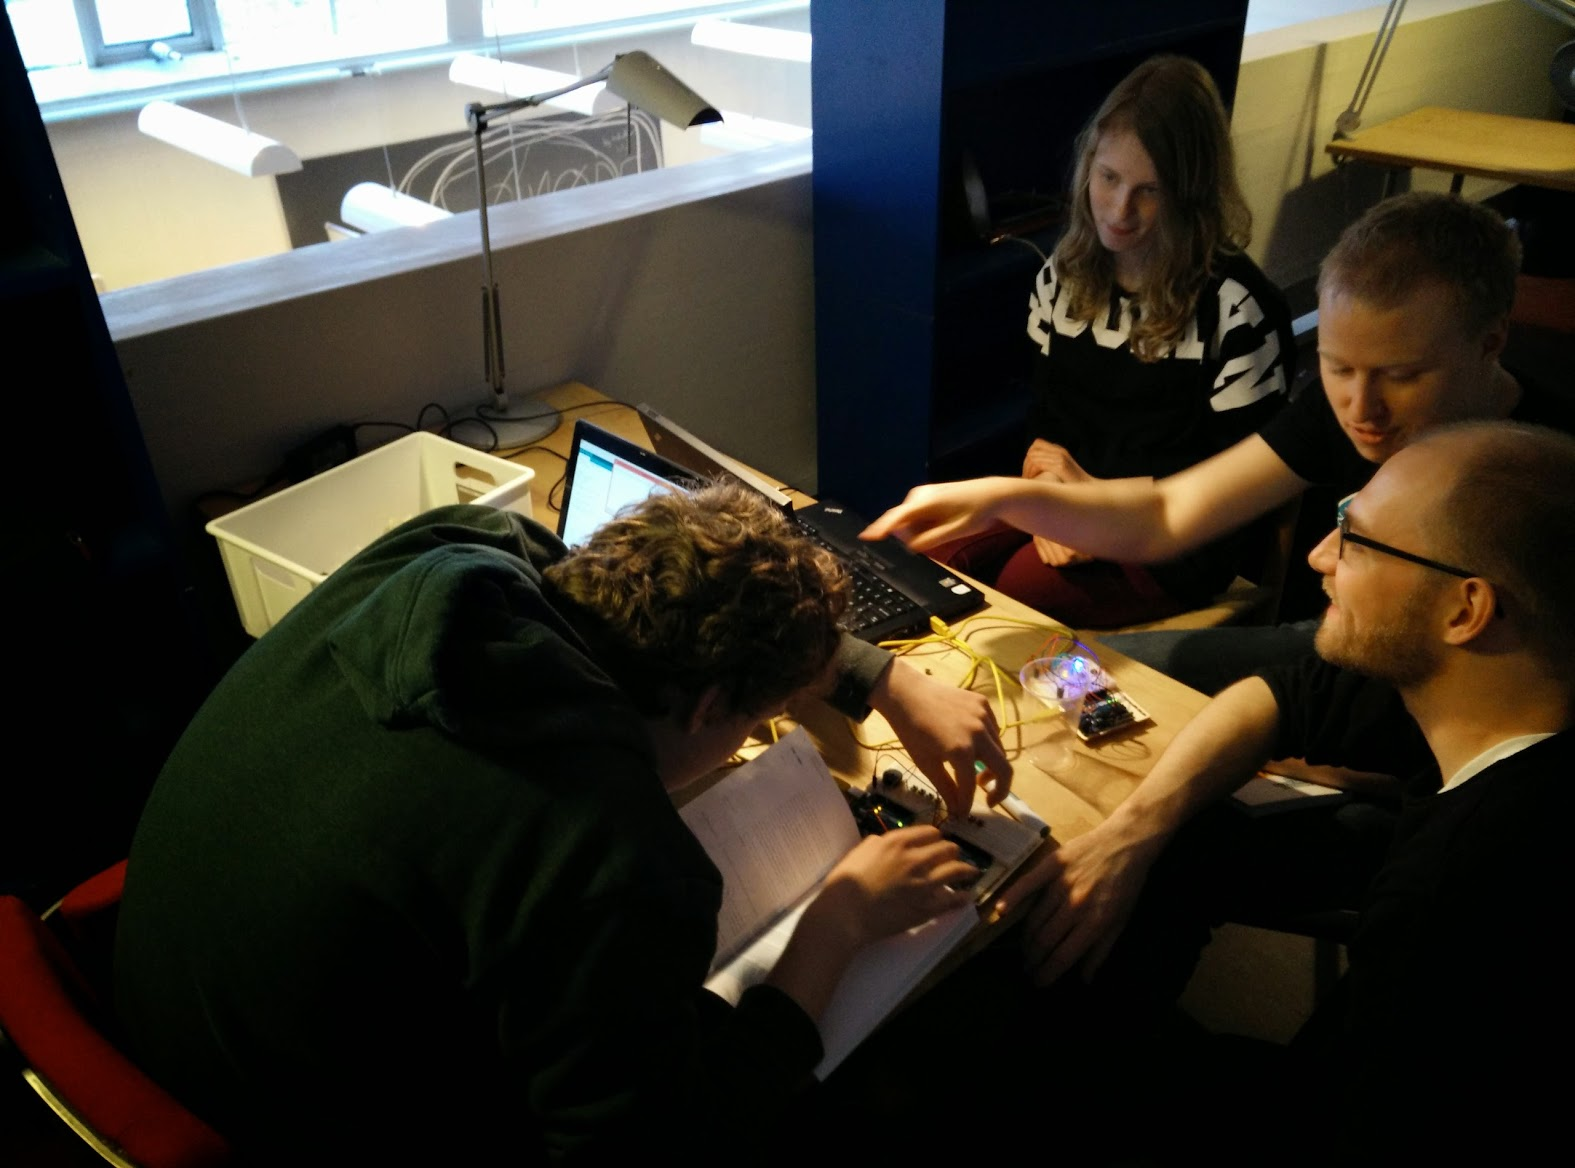
\includegraphics[width=\textwidth]{imagery/arduino-workshop}
\end{frame}

\begin{frame}
 \vspace{5mm}
 \includegraphics[width=\textwidth]{imagery/august-mindstorms}
\end{frame}

\begin{frame}
 \vspace{5mm}
 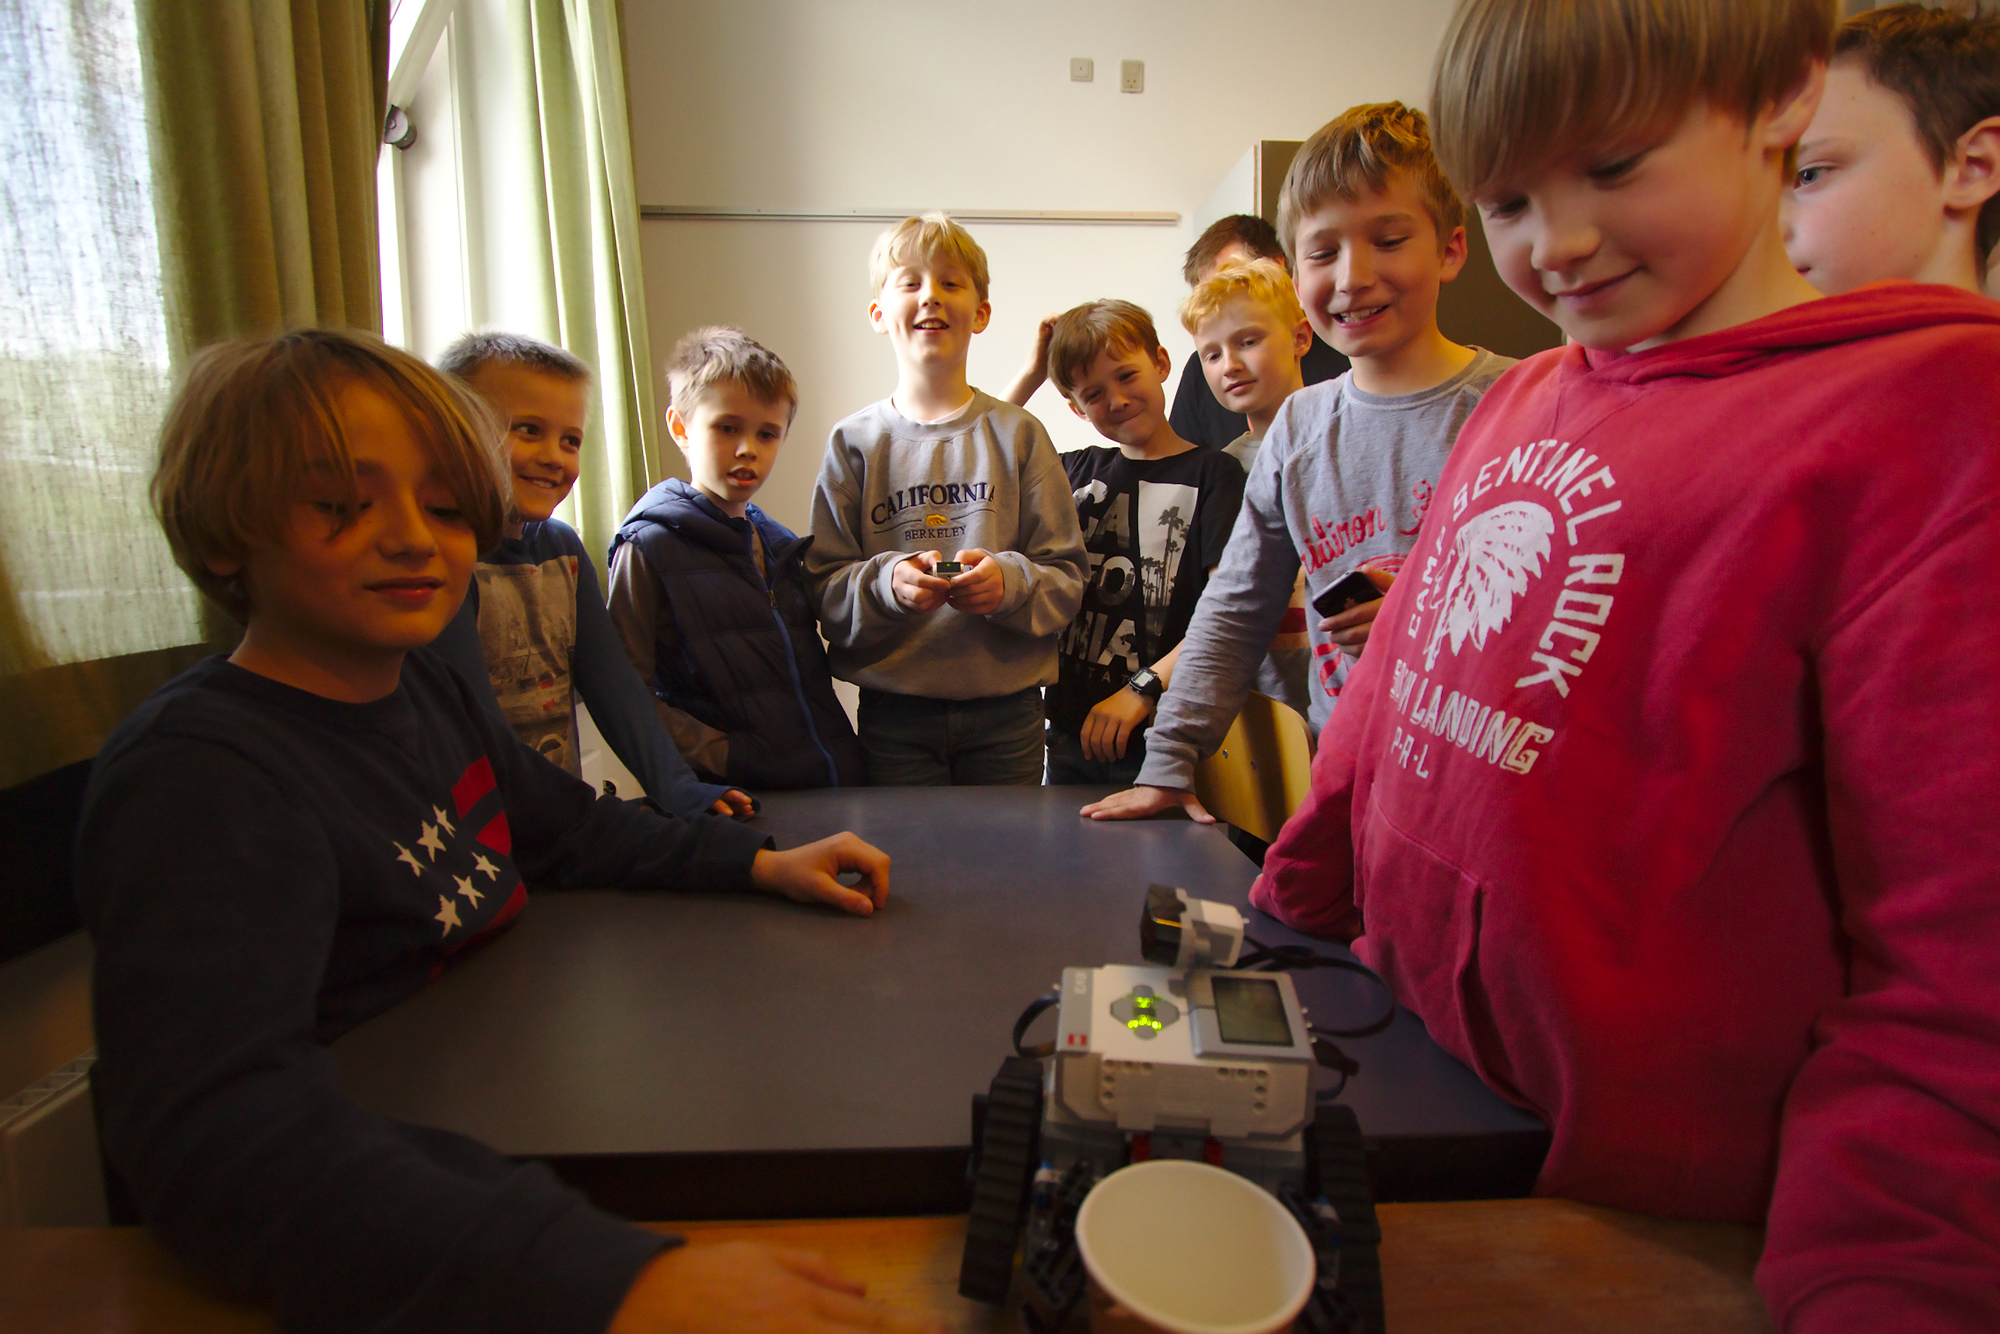
\includegraphics[width=\textwidth]{imagery/mindstorms-presentation}
\end{frame}

\begin{frame}
 \vspace{5mm}
 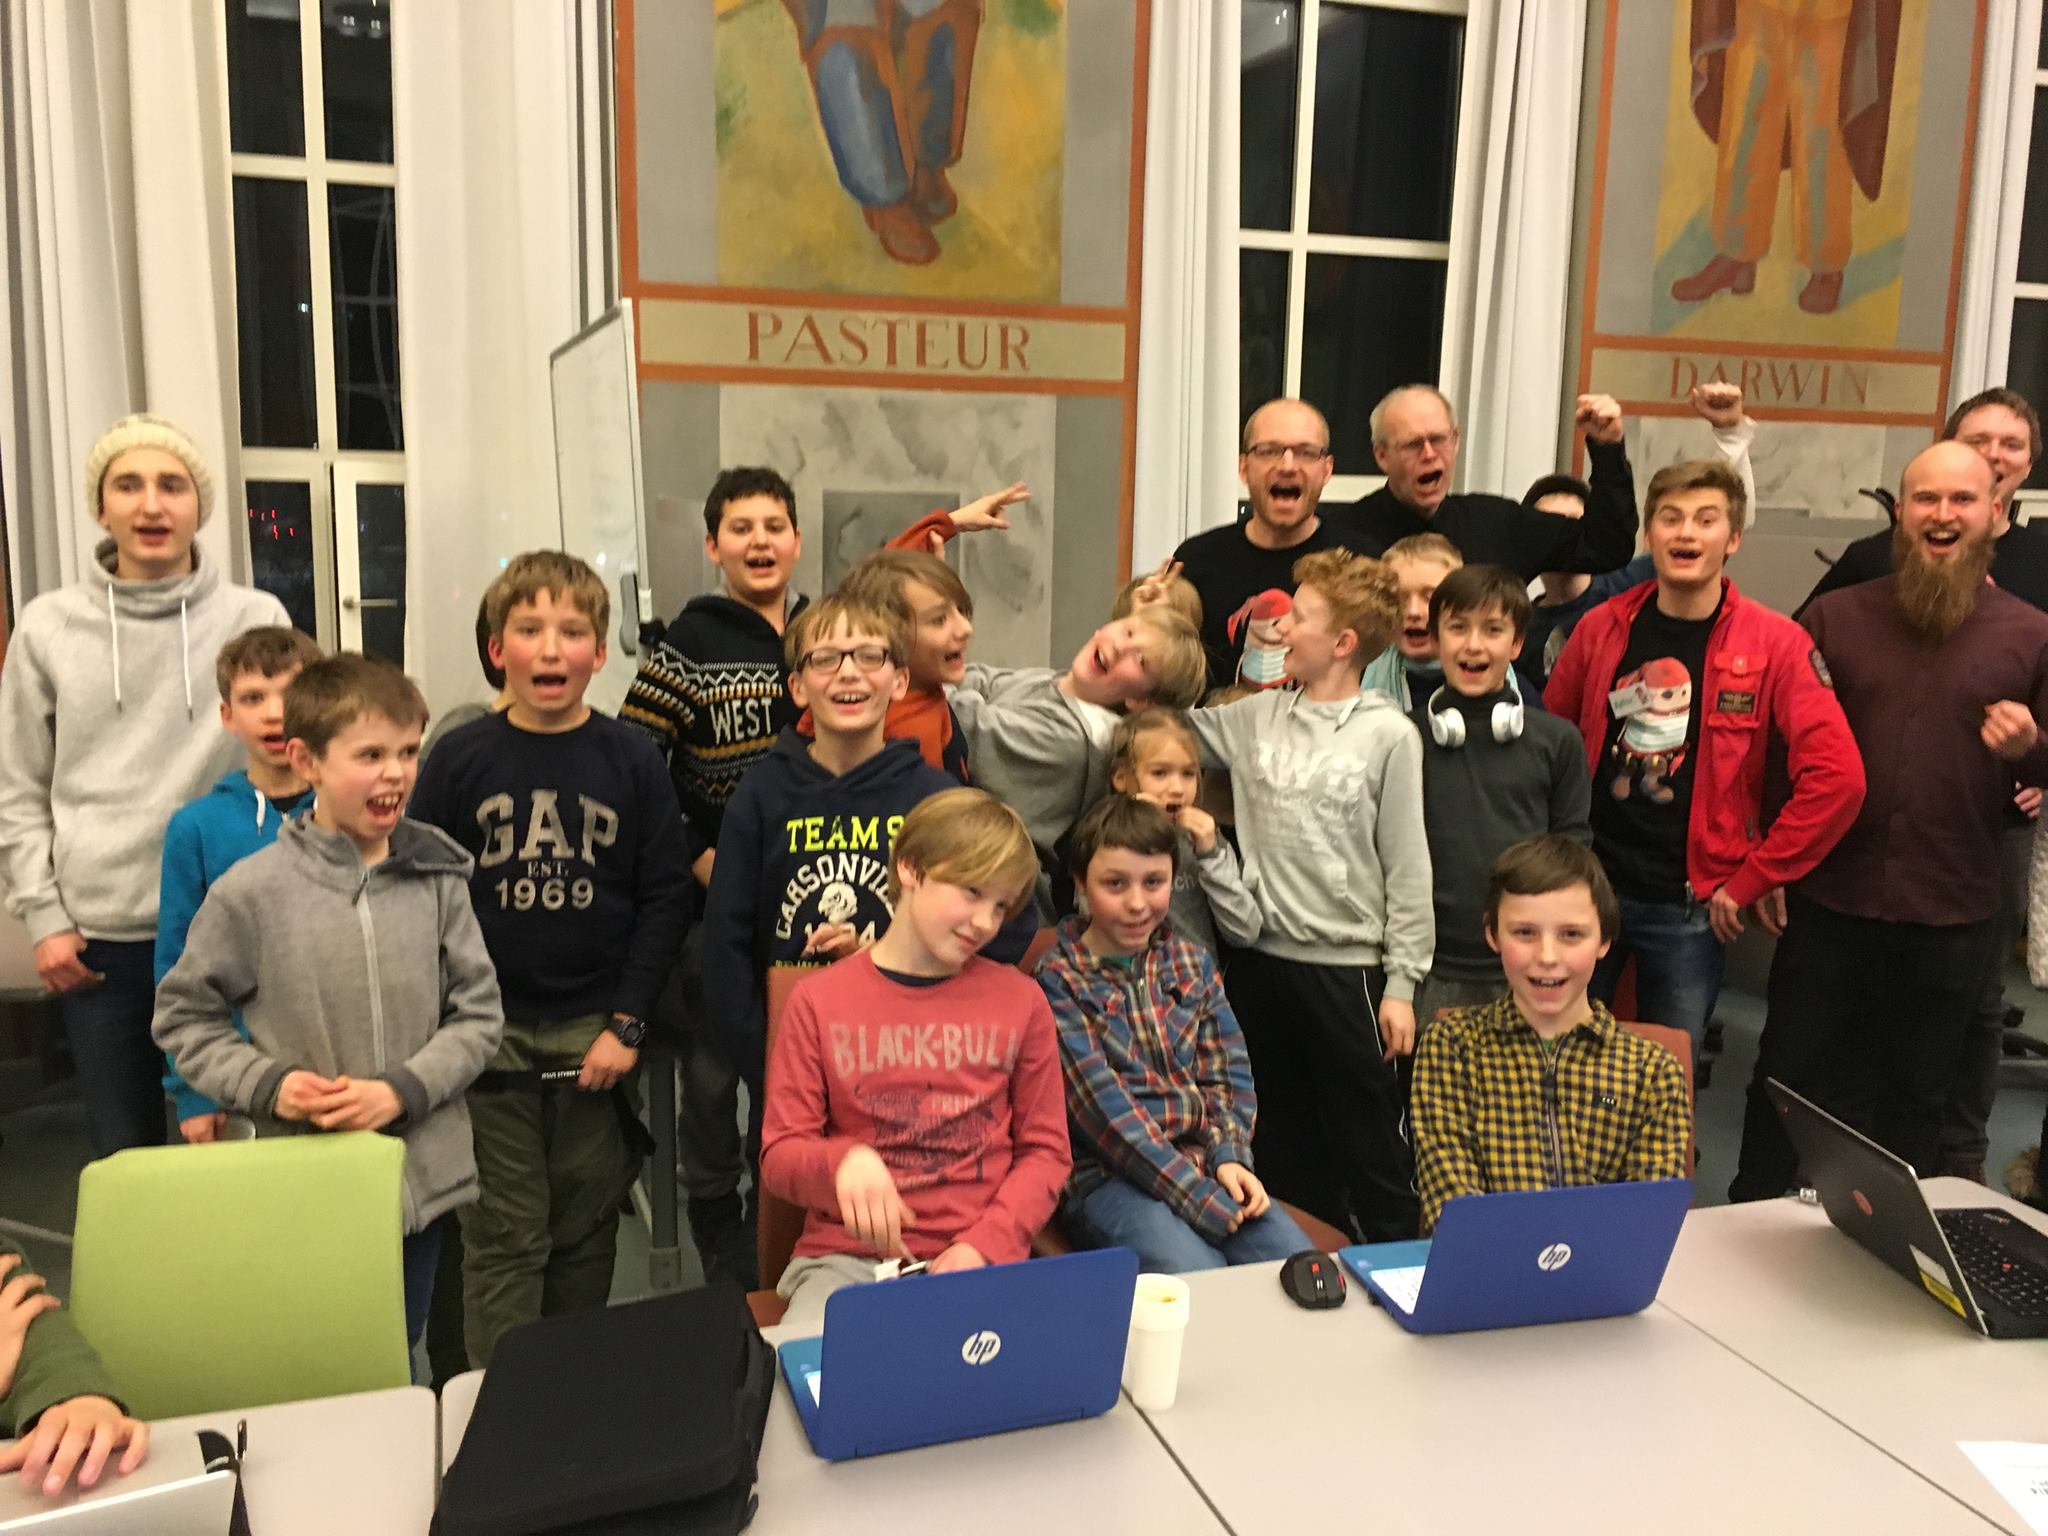
\includegraphics[width=\textwidth]{imagery/cpdiku}
\end{frame}



% \begin{frame}
% \frametitle{Scratch 4 Arduino}

% \end{frame}

% \section{Processing(.js)}
% \begin{frame}
% \frametitle{Processing(.js)}

% \end{frame}

% \subsection{... and other technologies}
% \begin{frame}

% \frametitle{Other technologies used}
% \todo{find logos}

% \begin{itemize}
% \item Processing(.js) via KhanAcademy
% \item Arduino
% \item Blender (3D modelling)
% \item Unity (2D and 3D games)
% \item LEGO Mindstorms and LEGO WeDo (expensive)
% \item littleBits (expensive)
% \end{itemize}
% \end{frame}

\begin{frame}
  \frametitle{Robot-sumo}
  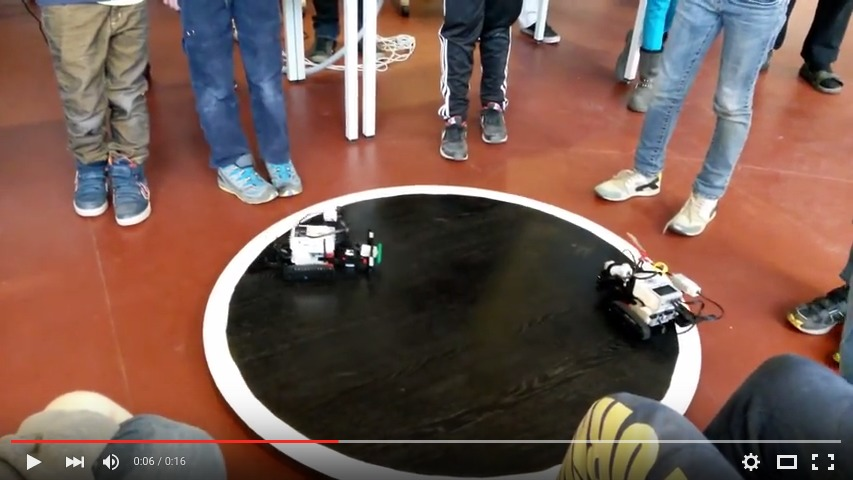
\includegraphics[width=\textwidth]{imagery/robotsumo}
  
  \url{https://www.youtube.com/watch?v=qcWTpXh-rOw}
\end{frame}

% \begin{frame}
%   \frametitle{Some processing example}
%   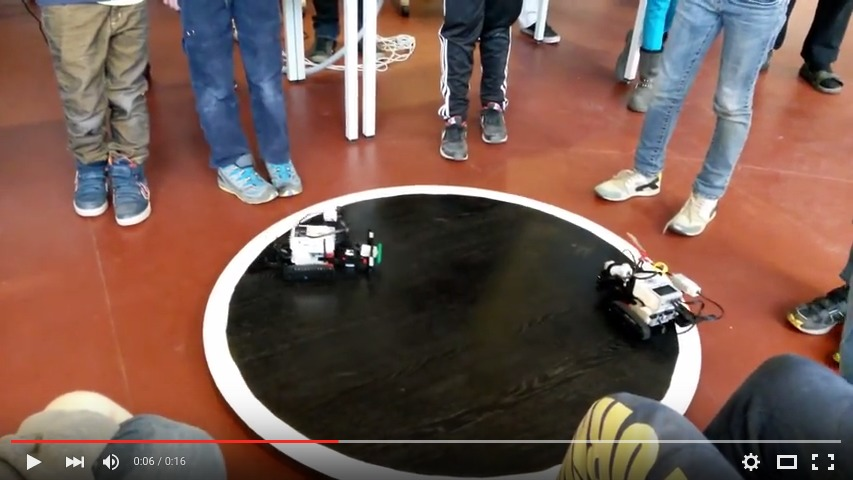
\includegraphics[width=\textwidth]{imagery/robotsumo}
  
% %  \url{https://www.youtube.com/watch?v=qcWTpXh-rOw}
% \end{frame}


\subsection{Difficulties ahead}
\begin{frame}
\frametitle{Difficulties}
\begin{itemize}
\item Few from age 14 and up
\item Few girls
\item Fostering friendships is hard, but important
  \begin{itemize}
  \item Force pair programming?
  \end{itemize}
\item Further education of volunteers
\end{itemize}
\end{frame}

\begin{frame}
  \frametitle{Age and gender (including waiting list)}
  \centerline{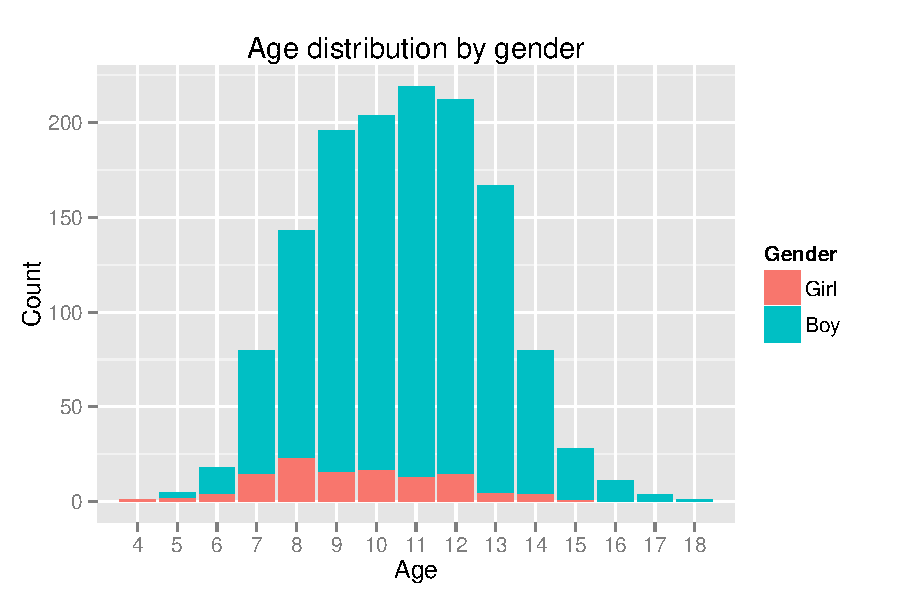
\includegraphics[width=\textwidth]{../datacrunching/age-gender-hist}}
\end{frame}

\begin{frame}
  \frametitle{Percentage of girls by age (including waiting list)}
  \centerline{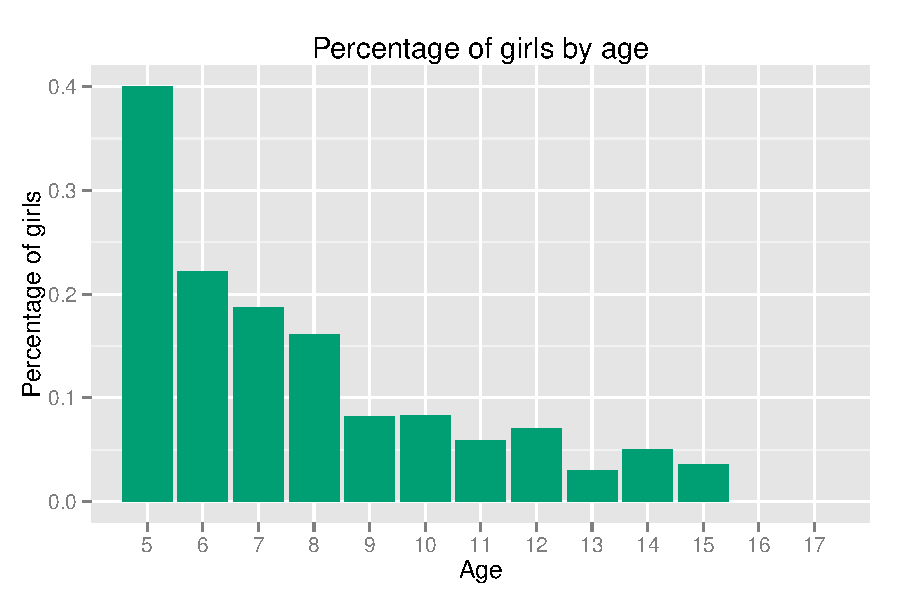
\includegraphics[width=\textwidth]{../datacrunching/girl_percentage}}
\end{frame}

\subsection{Volunteer Community}
\begin{frame}
  \frametitle{Volunteer community}
  \begin{center}
    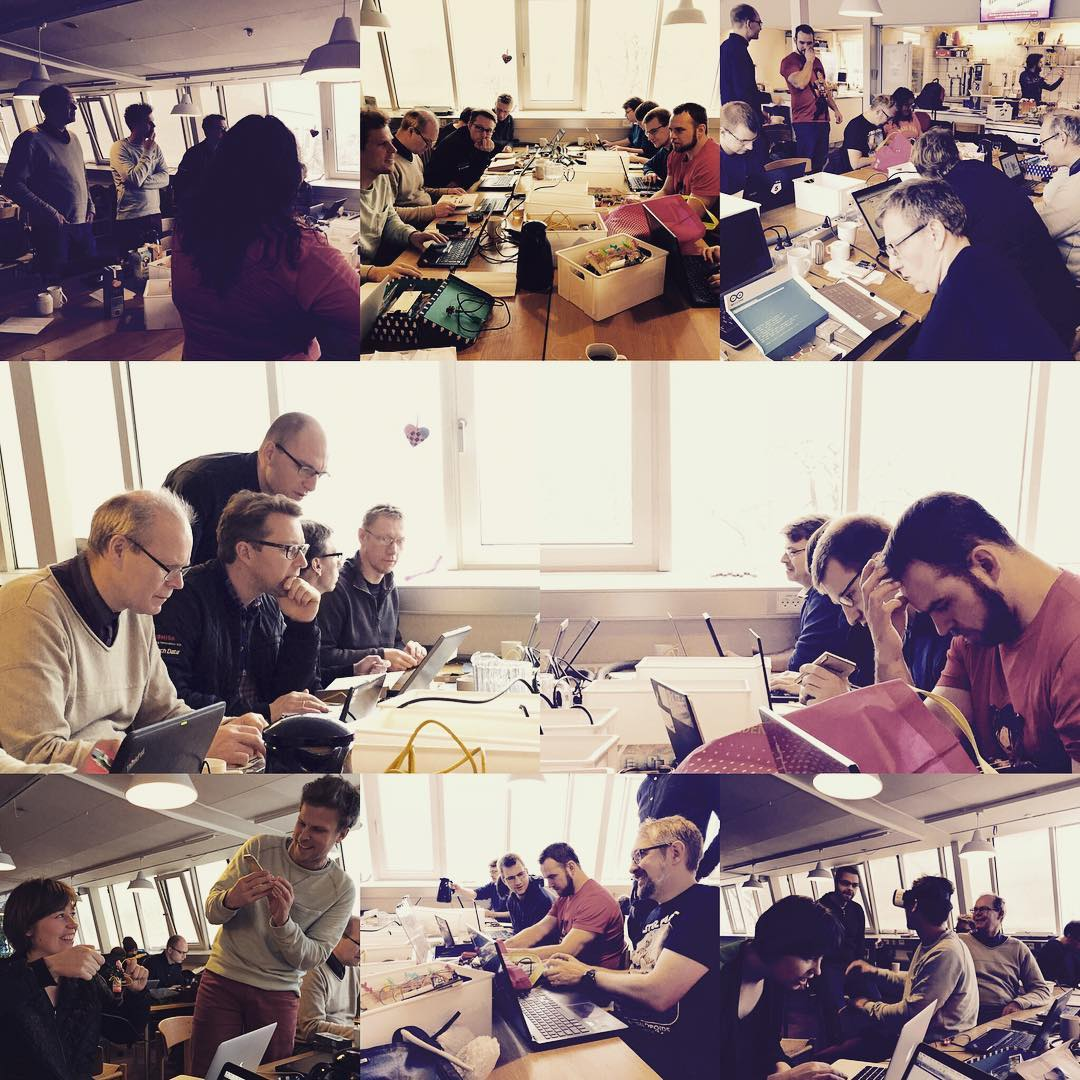
\includegraphics[width=0.7\textwidth]{imagery/2016-01-arduino-dag_DIKU.jpg}\\
    Arduino workshop for volunteers @ DIKU
  \end{center}

\end{frame}
% \begin{frame}
%   \frametitle{Volunteer community}
%   \begin{center}
%     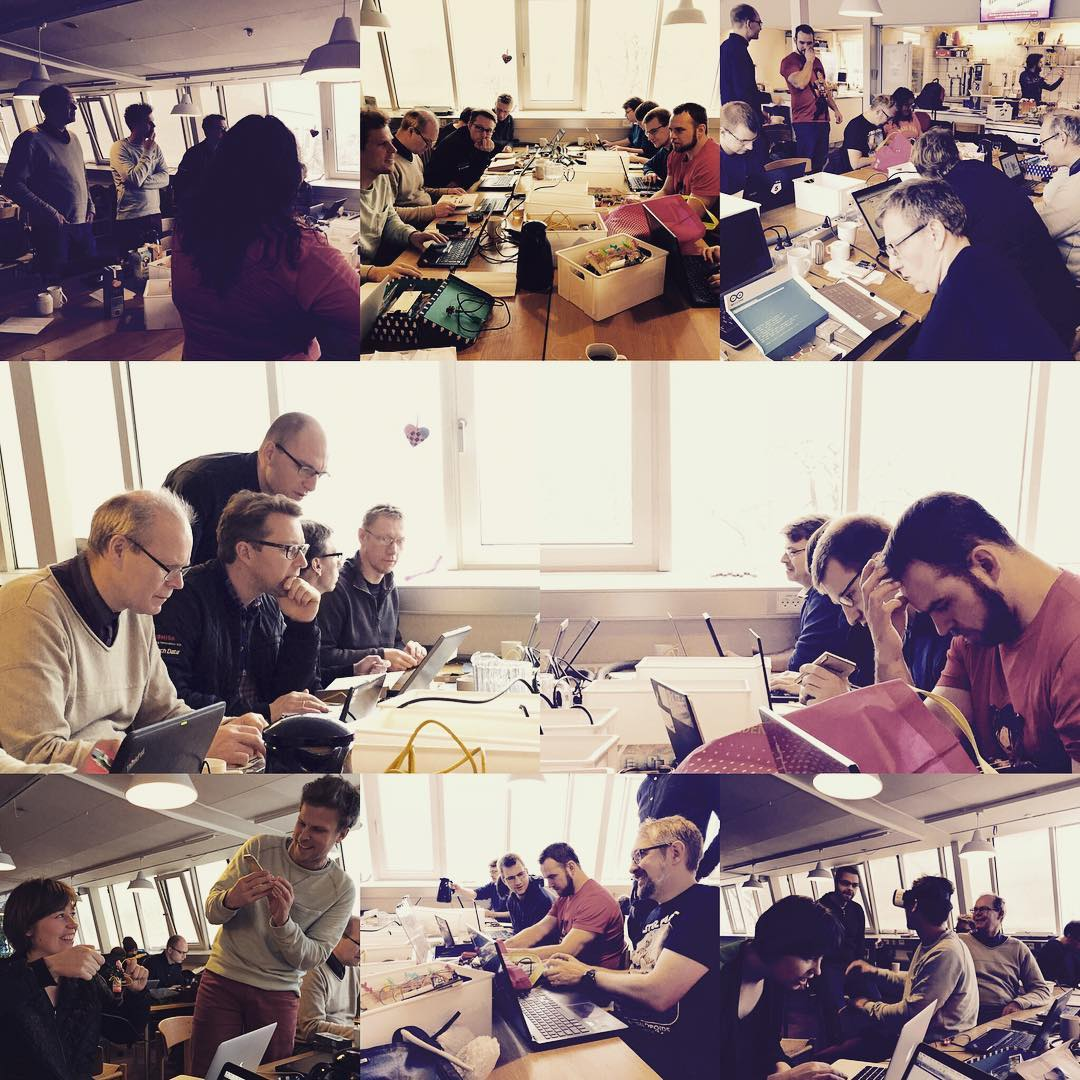
\includegraphics[width=0.7\textwidth]{imagery/2016-01-arduino-dag_DIKU.jpg}\\
%   \end{center}

% \end{frame}


% \section{Computing in schools}
% \begin{frame}
%   \frametitle{Computing in schools}
%   \begin{quotation}
%     "The computer is the Proteus of machines. Its essence is its
%     universality, its power to simulate. Because it can take on a
%     thousand forms and can serve a thousand functions, it can appeal
%     to a thousand tastes."

%     - Seymour Papert, in Mindstorms
%   \end{quotation}

%   We can already use this when teaching e.g. history, biology, chemistry,
%   or language classes!

%   \begin{itemize}
%   \item Make a game that teaches grade $N-1$ about photosynthesis
%   \item Make a game that teaches grade $N-1$ about life in ancient Rome
%   \item Make an interactive story that tells the story XYZ
%   \end{itemize}

%   More fun than a poster or a written report!
% \end{frame}

% \begin{frame}
%   \frametitle{But what do we want schools to teach?}

%   \begin{itemize}
%   \item Teach computing as a discipline, e.g. like math
%     \begin{itemize}
%     \item Algorithms vs. data
%     \item Systematic problem solving
%     \item Computational thinking
%     \end{itemize}
%   \item Teach computing as a craft/skill, e.g. like woodwork
%     \begin{itemize}
%     \item Focus on creation and tools
%     \item Creative and reflective thinking
%     \end{itemize}
%   \item A mix?
%   \item As a separate discipline or inside other classes?
%   \end{itemize}
% \end{frame}



\section{DIKU's involvement}
\begin{frame}
\frametitle{Why does a university use time teaching tweens and teens?}
\begin{itemize}
\item The teachers needs our expertise
\item Teacher education and re-education
\item Our connections to potential volunteers (alumni)
\item Getting at the table when defining how computing should be taught in schools
\item Potential research area
\item Influence on our own teaching practices
\end{itemize}
\end{frame}

\begin{frame}
  \frametitle{Research questions}

  \begin{itemize}
  \item How do you learn to program?
  \item What are the phases that learners go through?
  \item How do we best facilitate learning programming?
  \item Can programming be used to strengthen learning in other
    fields? % E.g. through programming simulations of ecosystems,
    % chemistry, etc.
  \item Can we observe the claimed benefits of computational thinking?
  \end{itemize}
\end{frame}



\begin{frame}
  \frametitle{Join us!}
  \begin{center}
    
\includegraphics[origin=c,angle=-20,width=0.7\textwidth]{imagery/wanted}
  \end{center}

\end{frame}

\end{document}